\documentclass[11pt]{report}
\usepackage[utf8x]{inputenc}
\usepackage{graphicx}
\usepackage{gensymb}
\usepackage{algorithm}
\usepackage[noend]{algpseudocode}
\usepackage{algpseudocode}
\graphicspath{ {./images/} }
\usepackage{fancyhdr}

\begin{document}
\title{\begin{figure}[htb]
\begin{center}

\includegraphics[width=8cm]{univ_logo}
\end{center}
\end{figure}SOEN 6011 : SOFTWARE ENGINEERING PROCESSES\\[.5em]
SUMMER 2022\\\vspace*{0.9in}
\begin{Large}
\textbf{ETERNITY} 
\end{Large}
\vspace*{0.9in}
\begin{Large}
\textbf{\\PROBLEM - 3} 
\\Pseudocode \& Algorithms\\
\end{Large}}
\author{By Prathika Anup Suvarna (40156790)}
\maketitle 
\pagenumbering{roman}
\setcounter{page}{0}

\tableofcontents
\pagebreak

\renewcommand{\thesection}{\arabic{section}}


\section{\Large \vspace{0.2 cm}Algorithms}
\pagenumbering{arabic}

\subsection{\Large \vspace{0.2 cm}Description}
To calculate the standard deviation for an array of numbers, there are two algorithms. In Algorithm 1, the standard deviation is usually calculated in two passes. In the first pass, we will find the mean and in the second pass, we will calculate the standard deviation of the numbers from the calculated mean. 
But we can do the same thing in one pass. So, Algorithm 2 do the same thing in one pass. It just rewrites the formula in a different way to calculate the mean and standard deviation in a single pass.

\subsection{\Large \vspace{0.2 cm}Decision on Psuedo-Code format}
There are two algorithms for which the psuedo code is provided below:-


\begin{algorithm}
\caption{Multi Pass Algorithm for calculating Standard Deviation}

\small
\begin{algorithmic}

\Function{StandardDeviation}{numArray[]}
\State $Sum \gets 0.0$

\State $Mean \gets 0.0$
\State $SD1 \gets 0.0$
\State $iLength \gets numArray.count()$
\For{$i = 0$ \textbf{to} $iLength$}
    \State Sum = Sum + numArray[i]
\EndFor    
\State $Mean= Sum/iLength$    
\For{$i = 0$ \textbf{to} $iLength$}
    \State diff = numArray[i]-Mean
    \State SD1 =SD1 + (diff*diff)
\EndFor
return SquareRoot(SD1 /iLength)
\EndFunction


\\
\Function{SquareRoot}{input}
\State $error \gets 0.00001$
\State $errorPrecision \gets 1$
\State $dup \gets input$
\State $iLength \gets numArray.count()$
\While{$errorPrecision > error$}
   \State $input = (input+dup/input)/2$
   \State $errorPrecision = input-dup/input$
\EndWhile
return input
\EndFunction
\\

\end{algorithmic}
\end{algorithm}
\pagebreak
\begin{algorithm}
\caption{Single Pass Algorithm for calculating Standard Deviation}


\begin{algorithmic}

\Function{StandardDeviation}{numArray[]}
\State $Sum \gets 0.0$

\State $Mean \gets 0.0$
\State $SD1 \gets 0.0$
\State $iLength \gets numArray.count()$
\For{$i = 0$ \textbf{to} $iLength$}
    \State Sum = Sum + numArray[i]
    \State SqSum = SqSum + (numArray[i]*numArray[i])
\EndFor    
\State $Mean= Sum/iLength$    
\State $Variance = SqSum/n - Mean*Mean$
\\
\quad\, return SquareRoot(SD1 /iLength)
\EndFunction


\\
\Function{SquareRoot}{input}
\State $error \gets 0.00001$
\State $errorPrecision \gets 1$
\State $dup \gets input$
\State $iLength \gets numArray.count()$
\While{$errorPrecision > error$}
   \State $input = (input+dup/input)/2$
   \State $errorPrecision = input-dup/input$
\EndWhile
return input
\EndFunction
\\

\end{algorithmic}
\end{algorithm}


\section{Multi-Pass VS Single Pass Algorithm}

\subsection{\Large \vspace{0.2 cm}Advantages}
\begin{itemize}
\item Multipass Algorithm 
\begin{itemize}
    \item It is most efficient algorithm to use.
    \item This algorithm is fast and can take collection of input data in the form of a file.
\end{itemize}

\item Singlepass Algorithm:-
\begin{itemize}
\item It is easy to understand.
\item The algorithm is taking up less time as there is only one iteration.
\end{itemize}
\end{itemize}

\subsection{\Large \vspace{0.2 cm}Disadvantages}
\begin{itemize}
\item Multipass Algorithm 

\begin{itemize}
    \item It will be difficult to develop in any other language.
    \item Memory stack will get full as it is using recursion and not iteration.
\end{itemize}

\item Singlepass Algorithm:-
\begin{itemize}
\item It gives inaccurate result when the array contains large numbers.
\item If there are more input data then this algorithm takes more time.
\end{itemize}
\end{itemize}

\section{Mindmap}
\begin{center}
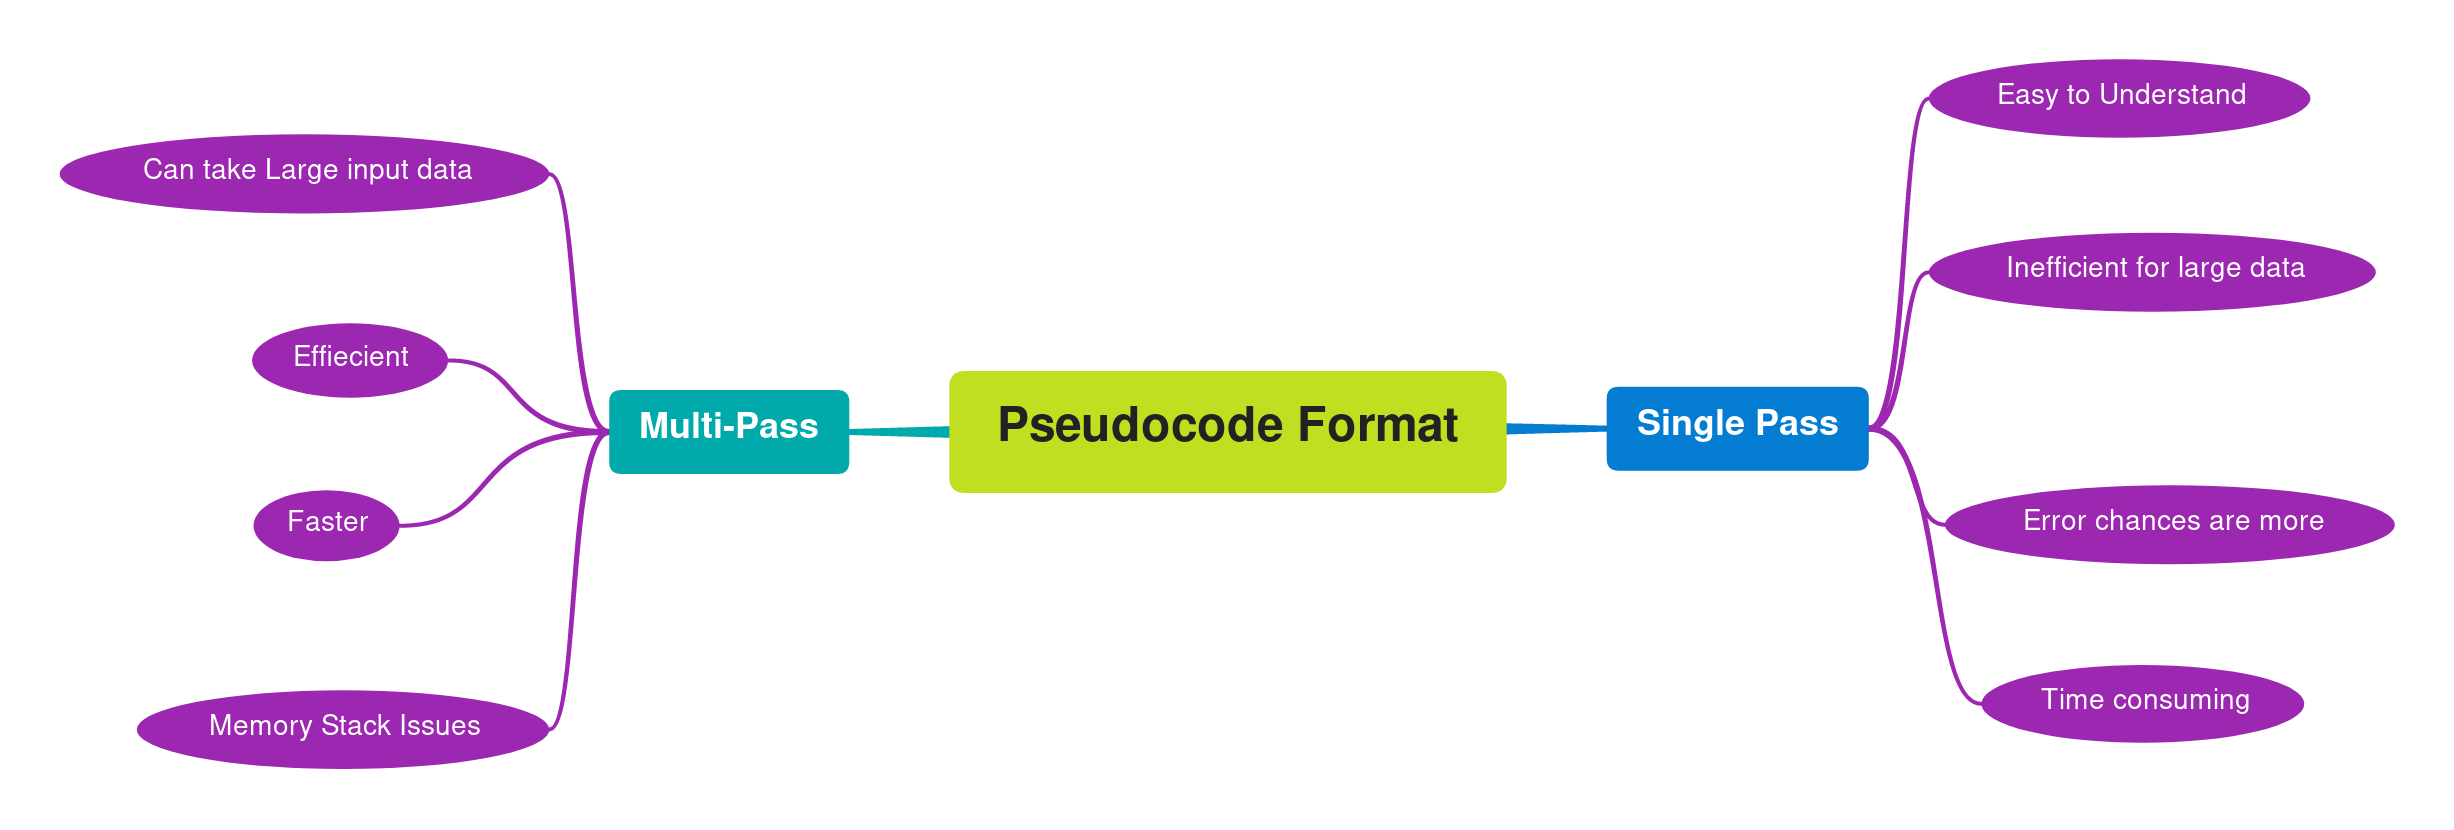
\includegraphics[width=15cm,height=8cm]{Mindmap}
\end{center}


\begin{thebibliography}{9}
\bibitem{Peter Kankowski}
Peter Kankowski
\\\texttt{https://www.strchr.com/standard\_deviation\_in\_one\_pass?allcomments=1}

\bibitem{Standard Deviations and Standard Errors} 
Standard Deviations and Standard Errors,
\\\texttt{https://www.ncbi.nlm.nih.gov/pmc/articles/PMC1255808/}


\end{thebibliography}



\end{document}